\documentclass[PhD]{dukethesis2006}

%preamble here for options

%-----------------------------------------------------------------------------%
% DEFINITIONS:
%
% include \usepackage here
%-----------------------------------------------------------------------------%
\usepackage{amsmath}
\usepackage{amssymb}
\usepackage{amsthm}
\usepackage{array}
\usepackage{epsfig}
\usepackage{graphicx}
\usepackage{xy}
\usepackage{etoolbox}


%----  macros to save typing; added by hartley, 2002 ----
\newcommand{\fig}{\begin{figure}[htbp]\centering}
\newcommand{\pic}[1]{\includegraphics[width=#1]}
\newcommand{\efig}{\end{figure}} 
%\newcommand{\efig}{\end{figure} \clearpage}
% Use \clearpage to cure ``too many floats'' problem (1 fig. per page).
\newcommand{\fr}[1]{Figure \ref{fig:#1}}
\newcommand{\FR}[1]{Figure \ref{fig:#1}}
\newcommand{\er}[1]{equation \ref{eq:#1}}
\newcommand{\ER}[1]{Equation \ref{eq:#1}}
\newcommand{\eq}{\begin{equation}}
\newcommand{\eeq}{\end{equation}}
\newcommand{\eqa}{\begin{eqnarray}}
\newcommand{\eeqa}{\end{eqnarray}}
\newcommand{\etal}{\nobreak\mbox{\it et al.}}



\newcommand{\singlespacing}{%
  \let\CS=\small\renewcommand{\baselinestretch}{1.0}\CS}
\newcommand{\doublespacing}{%
  \let\CS=\small\renewcommand{\baselinestretch}{1.6}\CS}
\newcommand{\normalspacing}{\doublespacing}

%\newcommand{\singlespacingplus}{%
%  \let\CS=\@currsize\renewcommand{\baselinestretch}{1.25}\tiny\CS}
%\newcommand{\realdoublespacing}{%
%  \let\CS=\@currsize\renewcommand{\baselinestretch}{2}\tiny\CS}
%\newcommand{\footnotespacing}{\singlespacing}
%\newcommand{\changespacing}[2]{%
%  \renewcommand{#1}{%
%    \let\CS=\@currsize\renewcommand{\baselinestretch}{#2}\tiny\CS}%
%}
%\newcommand{\changenormalspacing}[1]{\renewcommand{\normalspacing}{#1}}




%---- units ----
\newcommand{\days}{\nobreak\mbox{$\;$days}}
\newcommand{\hrs}{\nobreak\mbox{$\;$hrs}}
\newcommand{\mins}{\nobreak\mbox{$\;$min}}
\newcommand{\s}{\nobreak\mbox{$\;$s}}
\newcommand{\ms}{\nobreak\mbox{$\;$ms}}
\newcommand{\us}{\nobreak\mbox{$\;\mu$s}}
\newcommand{\inch}{\nobreak\mbox{$\;$in}}
\newcommand{\meter}{\nobreak\mbox{$\;$m}}
\newcommand{\cm}{\nobreak\mbox{$\;$cm}}
\newcommand{\mm}{\nobreak\mbox{$\;$mm}}
\newcommand{\um}{\nobreak\mbox{$\;\mu$m}}
\newcommand{\nm}{\nobreak\mbox{$\;$nm}}
\newcommand{\cmpers}{\nobreak\mbox{$\;$cm\,s$^{-1}$}}
\newcommand{\mmpers}{\nobreak\mbox{$\;$mm\,s$^{-1}$}}
\newcommand{\umpers}{\nobreak\mbox{$\;\mu$m\,s$^{-1}$}}
\newcommand{\g}{\nobreak\mbox{$\;$g}}
\newcommand{\kg}{\nobreak\mbox{$\;$kg}}
\newcommand{\hz}{\nobreak\mbox{$\;$Hz}}
\newcommand{\mhz}{\nobreak\mbox{$\;$mHz}}
\newcommand{\uhz}{\nobreak\mbox{$\;\mu$Hz}}


%---- oft-used complicated symbols ----
\newcommand{\rms}{\nobreak\mbox{$\sigma_{rms}$}}
\newcommand{\sat}{\nobreak\mbox{$\sigma_{\textrm{sat}}$}}
\newcommand{\DG}{\nobreak\mbox{$\Delta G^2$}}
\newcommand{\DS}{\nobreak\mbox{$\Delta\sigma$}}
\newcommand{\DQ}{\nobreak\mbox{$\Delta\theta$}}
\newcommand{\DSDQ}{\nobreak\mbox{$\Delta\sigma/\Delta\theta$}}
\newcommand{\dq}{\nobreak\mbox{$d\theta$}}
\newcommand{\ds}{\nobreak\mbox{$d\sigma$}}
\newcommand{\dsdq}{\nobreak\mbox{$d\sigma/d\theta$}}
\newcommand{\YY}{$\curlyvee\curlywedge$}
\newcommand{\GG}{\nobreak\mbox{$G^2$}}

 
% This is where the shortened versions of Latex environments like figure, equation, etc 
% are defined. See the file for the shortcuts.

\author{[Author Name]}
\advisor{[Advisor Name]}
\member{[Committee Member Name]}
\member{[Committee Member Name]}
\member{[Committee Member Name]}
\member{[Committee Member Name]}

\department{[Department Name]}
%\subject{xxx} If this is used, "subject" has to be un-commented in the cls file in several places
\title{[Dissertation Title]}

%end of preamble, beginning of printable document

\begin{document}


\Copyright

\maketitle

\makeabstract

\abstract

%An abstract is only required in doctoral dissertations. Your complete abstract should be no more than 350 words. In the abstract, you must (1) present the problem of the dissertation, (2) discuss the materials and methods used, and (3) state the conclusions reached. Individual chapters should not have abstracts. The Abstract will be published in Dissertation Abstracts International. Note that this should be the first numbered page: it is page iv; pages i, ii and iii  (copyright, dissertation signature page and abstract signature page) were counted but not numbered. If you look ahead, you will see that numbering up to the first page of text is in roman numerals. On the first page of text in chapter one, numbering restarts at 1. This numbering (1,2,3,4�%) is consecutive through the rest of the document. 

\acknowledgements
%Hosana pronomeca nelimigita ido ko, us negi lanta leterskribi mal. Re nia panjo alikvante nombrovorto, via tc bisi hekto koruso. Cii go unun oble drumo. Ke ties okej laringalo mia, anti duona alial ing fi. Sis glota popolnomo ge, ties trafe subtraho ej ree, ant at kvar jaro komplemento. It sor tempa oktiliono antaupriskribo.
%
%Modo tiela us cii, ne ehe intere rilativo. Ferio multiplikite id ajn. Tiele nenio akuzativa co ian. Unu ilia longa leteri op, vola hola ge cit, altmontaro kromakcento mi des. Ont lo grupo sezononomo, um kaj elparolo sanskrito.


%A table of contents file is automatically generated in the same folder as the .tex file when
%the \tableofcontents is used
\tableofcontents


%-----------------------------------------------------------------------------%
% replace FILE in \input{FILE} with name of tex file
% containing the given chapter, eg. for the introduction one could
% have FILE = intro if stored in intro.tex (.tex extension is assumed!).
%-----------------------------------------------------------------------------%

\chapter{Introduction}
\doublespacing
\pagenumbering{arabic}

%A large document requires a lot of input. Rather than putting the whole input in a single large file, it's more efficient to split it into several smaller ones. Regardless of how many separate files you use, there is one that is the root file; it is the one whose name you type when you run LaTeX. In this template, the introduction chapter is an external file (intro.tex) and the second chapter is contained internally in the root file (in this file you are reading)

\hypertarget{introduction}{%
\chapter{Introduction: the Deliberativist Stance}\label{ch:introduction}}
\pagenumbering{arabic}
\hypertarget{overview}{%
\section{Overview}\label{overview}}

In this dissertation, I defend the thesis that an epistemic judgment of
probability must be interpreted against the background of the
\emph{context of inquiry} in which it is made: in the \emph{abductive} context,
judgments of probability are matters of \emph{decision}, made
strategically in service to the investigative goal of the inquirer; in
\emph{deduction}, probabilities are \emph{derived} mathematically based on the
premises chosen in abduction, in order to explicate the implied
commitments the agent may incur from those decisions; during the
\emph{inductive} stage, the inquirer is expected to conduct her empirical
investigation in a deliberate manner, in accordance with the assertions and
decisions she made during abduction and deduction, collectively referred
to as the \emph{deliberative context}.

In order to explore this particular notion of \emph{abduction} in the
context of formal epistemology, I will critically examine the
\emph{Reflection Principle}, proposed by Bas van Fraassen, as a guiding
principle of epistemic rationality. The principle, roughly, says that my
degrees of beliefs \emph{now} are rationally constrained by what I think
my future degrees of beliefs \emph{will be}. If you think tomorrow you
will judge that your degree of belief for rain is, say, \(0.5\), it
would be irrational, the principle says, to assert that your \emph{current}
probability for the same event is anything other than \(0.5\).

To demystify Reflection and illuminate its connection to abduction, I
will devote chapter 2 to explaining van Fraassen's probabilist position
called \emph{voluntarism}. Essentially, voluntarism rejects the Bayesian
idea that judgments of probability are \emph{descriptive} reports of the
agent's psychological states. Instead, the voluntarist holds that to hold
a belief, partial or otherwise, is a matter of making a commitment to
stand by the belief in the future. It is, in a philosophically important
sense, analogous to making a \emph{promise}, which implies the
promisor's commitment to act in accordance with the content of the promise in the future. Thus, judgments of probability, like making promises, are what philosophers of language called \emph{speech acts}. To make the connection
between Reflection and abduction, I will provide a \emph{pragmatic}
interpretation of voluntarism by appealing to Peirce's later
formulation of the Pragmatic Maxim, according to which the practical difference implied by the acceptance of a belief is understood in terms of the contribution the belief makes to the agent's \emph{deliberate conduct}.

In chapter 3, I will discuss this idea of deliberate conduct in the
context of philosophy of statistics. One of the many disagreements
between the Bayesians and frequentists is the relevance of the so-called
``stopping rules'', which designate when sampling will be stopped.
Traditionally, Bayesian statisticians argue that stopping rules are
problematic, because they take into consideration extra-statistical
facts, specifically the agent's intention to stop. The thought is
that Bayesian methods count facts about the
experimenter's deliberations as irrelevant, due to the fact that Bayesians often accept the \emph{Likelihood
Principle}. I will argue that such an assumption is not correct: in
fact, like frequentists, Bayesians can also manipulate the statistical
result by changing their intentions to stop. I will propose that the
flight from intentions is not warranted; instead, we need a
philosophical account of how intentions are subject to rational
evaluation in terms of epistemic commitments and obligations. I will
introduce the problem of stopping rule in a historical context, and also consider a potential
objection to my argument based on a result regarding the value of
information proven by Frank Ramsey and I. J. Good.

One improvement of Reflection I will propose is that the commitment one
incurs from making an epistemic judgment ought to be understood not as
an unwavering perseverance in one's belief, but a deliberately structured disposition with
degrees of responsiveness to new experience. In other words, evidential
weight is a measure of one's \emph{dispositional commitment}: to put
oneself under the obligation to revise one's belief under different
evidential scenarios in a \emph{self-controlled} manner. Roughly, what I
mean is this: there are two senses in which my judgment that there is
a \(50/50\) chance that it will rain tomorrow has repercussion on our conduct in light of future evidence. One
is to say I have the obligation to hold steadfastly to the belief, even
if I come to encounter evidence that suggests the contrary. On a rigid
understanding of the idea that accepting a belief is a commitment, this
might sound like the thing to do. The other, one that I think makes more
sense in the context of inquiry, is this: I incur a particular
\emph{vulnerability} to evidence. For instance, my commitment may be
such that though at this point my personal probability of rain is
\(0.5\), I am willing to revise my opinion based on a small amount of
evidence. This could be the commitment I ought to have if I had no reason to
think one way or another, so that some evidence pointing to one way or
another is sufficient for me to be swayed. On the other hand, my
commitment to the probability of rain being \(0.5\) could be
\emph{weighty}: perhaps two meteorologists that I trust equally are each
giving completely conflicting forecasts, such that I am in a state of
ambivalence that cannot be easily resolved unless I find substantial
evidence to disqualify one of my sources as reliable. Reflection, for
the most part, does not address this. This will the be focus of chapter
4, in which I exploit the notion of the \emph{weight of evidence} in
explaining my proposal.

\hypertarget{historical-context}{%
\section{Historical Contexts and Motivations}\label{historical-context}}

How should probability constrain our beliefs? Can degrees of belief be
rational? These questions are central to philosophical problems that concern me in this dissertation. The dynamic between the freedom of thought and the security of logical thinking occupies an important role in the disagreement between the major historical figures.

\subsection{A Tale of Two Empiricisms}\label{empiricisms}


Historically, empiricism is often associated with a flavor of
foundationalism that holds that empirical evidence must in some sense be
untainted - if experience is to serve as the objective foundation of
knowledge, it must be unsullied by our attitudes, beliefs, and values.
It is without a doubt motivated by a conception of rationality familiar
to philosophers, because of Descartes' method of doubt:

\begin{quote}
Reason now leads me to think that I should hold back my assent from
opinions which are not completely certain and indubitable just as
carefully as I do from those which are patently false.\footnote{\cite{med}, 17.}
\end{quote}

The idea is that it is irrational to hold unjustified opinions, and the
empiricist response is to find a way in which our knowledge can be
justified by some indubitable experience. Quine is arguably the last
great empiricist in this tradition, even though it is not immediately
obvious. In ``Epistemology Naturalized'', Quine describes what he takes to
be `conceptual' and `doctrinal' cores of empiricist epistemology. The
conceptual core of empiricism, according to Quine, is concerned with the
explication of our concepts in terms of more ``basic'' concepts, which
refers directly to our sense experience, and the doctrinal side aims to
show that all of our justified beliefs can be inferentially traced to a
set of foundational and self-justified propositions.\footnote{\cite{epistnat}, 70--78.}
Even though Quine claimed to have jettisoned these traditional
empiricist commitments, and replaced them with a naturalized
epistemology, he never did abandon this empiricist project:
his idea of epistemology naturalized is simply to replace the
old-fashioned notion of ``experience'' with the physicalist equivalent that he
deemed more scientifically respectable. In his last major work, ``From
Stimulus to Science'', he still pursues the foundationalist project
under the guise of naturalism by suggesting ways in which the basis
of science can be reduced to the firing of neural receptors.\footnote{\cite{quinefromstim}, 15--16.}

Such an attitude also permeates through the works of Carnap, another
great empiricist. \emph{The Logical Structure of the World}, also known
by its German title \emph{Aufbau}, is often considered by Quine as the
most thorough attempt to carry out the project of reductionism, as its
aim is ``a step-by-step derivation or 'construction' of all concepts
from certain fundamental concepts\ldots{}''\footnote{\cite{aufbau} 5.}
Carnap the phenomenal reductionist---not necessarily the actual Carnap--- remained Quine's favorite philosophical
foil in virtually all of his work.

However, in the \emph{Aufbau} there is also an empiricist instinct that
is not antithetical to foundationalism but also emphasizes the role of
decision, intention, and volition in our practice of knowledge. Carnap explains that there
is nothing metaphysically necessary about his decision to choose sense experience as the basis for all concepts---its
appropriateness depends ultimately on the decider's
``standpoint.''\footnote{\cite{aufbau} 94--95.}

In \emph{The Logical Syntax of Language}, he codifies this normative
stance as \emph{the Principle of Tolerance}:

\begin{quote}
\emph{It is not our business to set up prohibitions, but to arrive at conventions\ldots{} In logic, there are no morals.} Everyone is at liberty to build up his own logic, i.e., his own form of language, as he wishes. All that is required of him is that, if he wishes to discuss it, he must state his methods clearly...\footnote{\cite{logicalsyntax}, 51--51.}
\end{quote}

This stance was evidently prompted by the disputes between logicians and
mathematicians regarding the ``correct'' language of logic. But the
standard of correctness does not exist until a language is chosen, so in
an important sense, trying to determine which language is better than
another is ultimately futile. However, once we adopt the Principle of
Tolerance, ``before us lies the boundless ocean of unlimited
possibilities.''\footnote{\cite{logicalsyntax}, xv, 50.} In ``Empiricism, Ontology, and Semantics,'' Carnap expresses this attitudes as the \emph{semantical method}, so-called because it takes the role of linguistic framework as central to the analysis of philosophical problems.\footnote{\cite{carnapsemantic}} In particular, Carnap argues that many philosophical questions needlessly arise due to confusions about questions internal to a framework and ones external to it. Carnap argues that many philosophical problems, including the existence of the external world, simply dissolve as soon as one recognizes that the choice of a framework is a pragmatic decision.

Carnap, I think, embodies two competing philosophical attitudes: one is
the desire for an algorithmic ideal of rationality that allows only  stepwise movement in the space of reasons, and the other is the
recognition that rationality permits leaps over epistemic gaps through extra-logical elements such as decisions and perspectives. The former point of
view demands clarity of thought, so that each inferential step is
perfectly secure. The second attitude, on the other hands, recognizes that the contributions of volition can never be wholly eliminated from our epistemic practice. Our inquiries often have to begin with assumptions that cannot be justified by the current body of evidence, but we must take a leap of faith with the hope that its provisional acceptance could lead the gain in knowledge or information.

The goal of this dissertation can be summarized as a philosophical
exploration of the dynamic between these two styles of thinking within
the context of probabilistic reasoning. My main contention is that both
philosophical attitudes are needed in order to make sense of our rationality, and
their interaction must be understood in the respective role they play in
the different \emph{contexts} of inquiry.

The notion of inquiry is an explicit reference to the philosophy of C.
S. Peirce, whose view is an important basis of and inspiration for the
position I aim to defend and develop here. Peirce, as I understand him,
has a systematic understanding of the context-sensitivity of epistemic
judgments. That is, the evaluation of an assertion or a belief cannot be
detached from the context in which it occurs: an assertion of
probability has different normative implications in the context of
abduction, deduction, and induction. My proposal is that an
assertion has no normative force unless it is underwritten by an
epistemic practice that incentivizes the agent to stand by the
obligations imposed upon her.

Neither Carnap nor empiricism play a explicit role in the position I endeavor to defend in this dissertation; however, the ineliminable volitional element in our empirical rationality is central to the core issues to be discussed in virtually every chapter. This is an especially important context to keep in mind in our discussion of van Fraassen, who makes explicit reference to Carnap's view on the role of decision in ``Empiricism, Ontology, and Semantics''\footnote{\cite{antinatural}, 83---84}. Van Fraassen's voluntarism, in particular, should be see as belonging to the same tradition of empiricism that I ascribed to Carnap earlier.




\hypertarget{rational-degrees-of-belief}{%
\subsection{Keynes and Ramsey on Rational Degrees of
Belief}\label{sec:rational-degrees-of-belief}}

Probability, in J. M. Keynes' view, is defined as a logical relation between
a premise and a conclusion. Probability relations are logical, because
this relation belongs to the same conceptual category as the entailment
relation between the premises and conclusion in a deductive argument.
Keynes says:

\begin{quote}
Inasmuch as it is always assumed that we can sometimes judge directly
that a conclusion follows from a premiss, it is no great extension of
this assumption to suppose that we can sometimes recognise that a
conclusion partially follows from, or stands in a relation of
probability to, a premiss.\footnote{\cite{keynes}, 57.}
\end{quote}

Keynes' logical interpretation of probability has the advantage of
providing a direct explanation of why probability is \emph{normative}:
we \emph{should} reason in accordance with probability for the same reason
that we should respect a deductive rule like \emph{modus ponens}: the
degrees of a person's partial belief should correspond to the degree to
which the premises render the conclusion probable, whereas in a
deductive proof, one has to accept the conclusion as necessarily true,
were the premises true. Hence Keynes talks about probability not as
something we can attribute to a proposition, nor one's attitude of it,
but a logical and objective property of an argument.\footnote{There is a technical
  consequence for this. If probability is a relation, it follows that it
  never makes sense to talk about the probability of an event without in
  relation to any other proposition, so for Keynes all probabilities are
  conditional probabilities.}

As frequentists often find little use for the idea of degrees of belief,
it is often seen as a notion exclusive to subjective theories of
probability; however, Keynes' rational degrees of belief are conceived to
be objective relations independent of the human mind. More important, in Keynes, we find the foundationalist attitude that he
inherited from the logical atomism of Russell. Keynes accepts Russell's
idea of knowledge by acquaintance: some propositions, such as ``I have a
sensation of yellow'', are justified by virtue of being perceptually
acquainted with it.\footnote{\cite{keynes}, 11--12.} Furthermore, acquaintance
yields not only knowledge of the senses, but also of logical relations:

\begin{quote}
When we know something by argument this must be through direct
acquaintance with some logical relation between the conclusion and the
premiss. In all knowledge, therefore, there is some direct element; and
logic can never be made purely mechanical. All it can do is so to
arrange the reasoning that the logical relations, which have to be
perceived directly, are made explicit and are of a simple
kind.\footnote{\cite{keynes}, 14.}
\end{quote}

This can be a puzzling position, considering Keynes' goal is to develop a
formal system of probability. The puzzlement can be formulated as follows: if logical relations are irreducible entities
knowable to us only by perception or intuition, then why would we need a
formal system? Keynes' answer is that everyone's intuitive faculty is
different---``the perceptions of some relations of probability may be
outside the powers of some or all of us'---so we need principles to make
these perception explicit and justified.\footnote{\cite{keynes}, 18.}

For instance, one's judgment of two events being equally probable could be mistaken, hence we need the important principle called the \emph{Principle of Indifference}. Laplace
is well-known for articulating a version of it:

\begin{quote}
When the probability of a simple event is unknown, one may suppose that
it is equally likely to take on any value from zero to one\ldots{} the
probability of each of these hypotheses, given the observed event, is a
fraction whose numerator is the probability of the event under this hypothesis, and whose denominator is the sum of similar probabilities under each of the hypotheses.\footnote{\cite{laplace}, 20.}
\end{quote}

In other words, when we are in complete ignorance regarding the outcome
of the event, the probability of each possible outcome is:

$$\frac{1}{\text{\# of total possible hypotheses}}$$

Many have criticized this principle. Peirce vehemently
rejects it, as he argues that in many cases, especially when the number
of possible outcomes is ambiguous, using the principle will lead to
contradictions.\footnote{\cite{probabilityofinduction}, section II}A simple example would be to determine the probability of an unknown object, for example, a marble, having a certain color, say, red. Suppose I have no information about this marble, so I have no
reason to think the marble is red or not.\footnote{Assume that the surface
  of a marble can only have one color.} Following the principle, it would
seem that \(P(R) = P(\neg R) = 0.5\). However, we are led to
contradictions when we asks if the marble is yellow, black, etc.; because,
using the same reasoning, we would say
\(P(Y) = P(\neg Y) = P(B) = P(\neg B) = 0.5\). The contradiction is that
these are mutually exclusive propositions, so axioms of probability say
that their sum cannot go beyond \(1\).

When Keynes wrote \emph{A Treatise on Probability}, he was keenly aware
of the paradoxes caused by the Principle of Indifference. However, he
thinks that the paradoxes suggest only that the principle is to be
restricted, not abandoned altogether. To begin, he notes that the
crucial terms used in the principle are not clearly defined:

\begin{quote}
The principle states that `there must be no known reason for preferring
one of a set of alternatives to any other.' What does this mean? What
are `reasons,' and how are we to know whether they do or do not justify
us in preferring one alternative to another? I do not know any
discussion of Probability in which this question has been so much as
asked.\footnote{\cite{keynes}, 58.}
\end{quote}

Instead, he proposes that the ambiguous clause ought to be explicated in terms of
\emph{conditional relevance}: 

\begin{quote}
This distinction enables us to formulate the Principle of Indifference at any rate more precisely. There must be no relevant evidence relating to one alternative, unless there is corresponding evidence relating to the other; our relevant evidence, that is to say, must be symmetrical with regard to the alternatives, and must be applicable to each in the same manner.	\footnote{\cite{keynes}, 61.}
\end{quote}


That is, to say that we have no reason to prefer
a proposition \(H\) over its alternatives is to say that there is no
evidence such that it is relevant to \(H\) but irrelevant to all the
alternatives. Roughly speaking, \(E\) is relevant to \(H\) on background
knowledge \(K\) if and only if: \[P(H|K) \neq P(H|K\wedge E)\] Thus, one necessary condition for a justified application
of Indifference is that for a set of \(n\) possible outcomes,
\(H_1,...H_n\), there is no evidential proposition \(E\) such that it is
conditionally relevant to some but not others. 

I will flag an important issue here. Keynes is not satisfied with this definition of relevance, because it fails to account for what he calls the \emph{weight} of the evidence.\footnote{\cite{keynes}, 79.} The basic idea is that some intuitively relevant evidence does not raise of lower the probability of the hypothesis it confirms. This will be discussed in chapter \ref{ch:woe}.

In any case, Keynes argues that the Principle of
Indifference should not be used when the alternatives under
consideration can be further analyzed, or, using his term,
``divisible''. Consider again the marble example. The paradox begins
with the assumption that red and not red are the two alternatives. While
it is true that these outcomes are exhaustive, ``not red'' should be
analyzed before we distribute the probabilities, since it also
encompasses the possibility that it is black, it is blue, etc. So
according to Keynes' conditions, judging \(P(R) = P(\neg R) = 0.5\) is
unjustified, since it is not a legal application of the Principle of
Indifference.

With Keynes' version of the principle, we have to know a great deal
about the setup of the sample space, before even entertaining the
possibility of indifference between alternatives. According to Keynes'
proposal, this means that most of our intuitive judgments of
indifference would be illicit. In fact, Keynes admits just as much: he
holds that in many, if not most, scenarios, the probability of a given
event cannot be given a precise value.\footnote{\cite{keynes},41-42.} For many propositions, it would
be impossible to say anything about their probability at all. Of course,
Keynes is not saying that it is psychologically impossible for us to
have degrees of belief for a proposition that fails to satisfy these
conditions, but he is saying that they would not be \emph{rational}
degrees of belief.

Keynes' epistemology behind his theory of probability presupposes a very restrictive view of how it means for a probabilistic judgment to be rational.  The Principle of Indifference serves as a compelling \emph{normative} principle that is required for any rational judgment of indifference. Because of Keynes' logical view of probability, to attribute equal probability between two outcomes without satisfying the principle would essentially the same as making an deductively invalid argument.\footnote{\cite{keynes}, 60.}
So, the principle serves as a standard of correctness by specifying the conditions under which the uniform distribution of probability among hypotheses is \emph{rational}, i.e., justified. This is very different than saying that, whenever you have no information about the problem, you are allowed to uniformly distribute your degrees of belief. On Keynes' view, you should only do so when you have enough information to know the indifference is warrant; otherwise, you should just \emph{withhold} your judgment.

In his ``Truth and Probability'', Ramsey responds to Keynes' view by
rejecting the conception of degree of belief as perceptible logical
relations:

\begin{quote}
\ldots{}there really do not seem to be any such things as the
probability relations {[}Keynes{]} describes. He supposes that, at any
rate in certain cases, they can be perceived; but speaking for myself I
feel confident that this is not true. I do not perceive them, and if I
am to be persuaded that they exist it must be by argument; moreover I
shrewdly suspect that others do not perceive them either, because they
are able to come to so very little agreement as to which of them relates
any two given propositions.
\end{quote}

However, part of the appeal of Keynes' theory is that probability itself
is irreducibly normative, since logical relations are objective and logical. It would seem that denying the existence of these logical relations also robs probability of its normative force. Ramsey recognizes this, and explicitly rejects both the Principle of Indifference and Keynes' strongly normative conception of rational degrees of belief. Keynes' position, Ramsey argues, \emph{requires} principles such as Indifference is that Keynes assumes that degrees of belief must be \emph{justified} before it can be admitted in the calculus of probability; however, Ramsey thinks that such a demand cannot be satisfied:

\begin{quote}
\ldots{}to ask what initial degrees of belief are justified\ldots{}
seems to me a meaningless question; and even if it had a meaning I do
not see how it could be answered.\footnote{\cite{ramsey}, 88.}
\end{quote}

Once this requirement of rationality is jettisoned,

\begin{quote}
the Principle of Indifference can now be altogether dispensed with; we
do not regard it as belonging to formal logic to say what should be a
man's expectation of drawing a white or a black ball from an urn; his
original expectations may within the limits of consistency be any he
likes; all we have to point out is that if he has certain expectations
he is bound in consistency to have certain others. This is simply
bringing probability into line with ordinary formal logic, which does
not criticize premisses but merely declares that certain conclusions are
the only ones consistent with them.
\end{quote}

Thus, Ramsey recognizes the normative nature of Keynes' use of the
principle: it constrains our beliefs such that when the conditions for
Indifference are met, one is required by rationality to assign equal probabilities to the outcomes. As the quotation above
makes clear, Ramsey's view makes no such demand. As far as he is
concerned, it is not probability's business to tell people what degrees
of belief they \emph{should} have. Instead, the normative force of
probability is the same as that of deductive logic: it serves as a tool
for checking the \emph{consistency} of  beliefs, and no more.

Ramsey, then, is advocating what came to be the standard notion of
Bayesian rationality: coherence. The question has shifted from ``what
are rational degrees of belief?'' to ``is this set of partial beliefs
consistent?'' Ramsey's analogy to deductive logic is helpful. Consider
this argument:

\begin{description}
	\item[Premise 1] All Chinese are Martians.
	\item[Premise 2]  Socrates is Chinese.
	\item[Conclusion] Socrates is Martian.
\end{description}

This is one of the first lessons every student from an introductory logic class would learn: even though the argument contains all false claims, from a deductive
perspective, it is a perfectly valid argument. In the same way, if we
have a definitely fair coin, yet the agent still decides that
\(P(Heads)=0.999\), she is still rational as long as she also believes
\(P(Tails) = 0.001\). This normative point is perhaps the most
influential among the ideas from ``Truth and Probability,'' as Ramsey
gestures toward the use of Dutch book arguments in support of coherence
as a requirement of rationality: anyone who violates the axioms of
probability ``could have a book made against him by a cunning bettor and
would then stand to lose in any event.''\footnote{\cite{ramsey}, 78} The argument
is based on the assumption that the agent's willingness to bet is tied to
her degrees of belief and utility function, so an inconsistent set of
partial beliefs would imply contradictory betting behavior that could be
exploited.

For instance, suppose the agent believe than \(P(Heads) = 0.999\) yet also
simultaneously holding that \(P(Tails) = 0.5\). This means, based on the
assumptions required by Dutch book arguments, one would be willing to
pay respectively \$0.999 and \$0.5 for a bet that pays \$1. So, if a
bookie offers the agent both bets at those prices, which comes to the
total of \$1.499, these bets should appear to be fair, based on her
degrees of belief. But she is guaranteed to lose money from this deal,
since landing on heads and on tails are mutually exclusive, she will win
at most \$1, so she lose \(1.499 - 1 = 0.499\) for sure. This is due to
the fact that she violates the axiom of probability that says that the
sum of the probability of each possible outcome has to be
\(1\).\footnote{\cite{hajekdutchbook}, 176.}

I do not wish to dispute the effectiveness of Dutch book arguments here. In section \ref{dutchbook-argument-for-reflection}, we will discuss one particular important use of the argument, but my thesis does not depend on it.
For now, let us for the sake of argument assume that probabilistic coherence is a
basic requirement of rationality. Still, there are aspects of probabilistic rationality  unaccounted for in Ramsey's view, even
if we grant the use of Dutch book arguments. Is coherence a
sufficient substitute for a normative conception of degrees of belief?
L. J. Savage, a strong advocate of Bayesianism and subjective
probability, expresses his doubts about this:

\begin{quote}
According to the personalistic view, the role of the mathematical theory
of probability is to enable the person using it to detect
inconsistencies in his own real or envisaged behavior. It is also
understood that, having detected an inconsistency, he will remove it. An
inconsistency is typically removable in many different ways, among which
the theory gives no guidance for choosing.\footnote{\cite{savage}, 57.}
\end{quote}

Savage's point can be illustrated by reconsidering the Dutch book case
above: suppose the agent is convinced that her degrees of beliefs,
\(P(Heads) = 0.999\) and \(P(Tails) = 0.5\) are incoherent: what
normative conclusion should she draw from this? The only advice coherence
could give is that the sum should add up to 1, but should she lower
\(P(Heads)\) to \(0.5\) or lower \(P(Tails)\) to \(0.001\)? In fact,
there are, quite literally, infinite ways to for her to resolve the
inconsistency. This illuminates the lacuna left open by a coherentist conception of probabilistic rationality, motivated by Ramsey's rejection of Keynes' rational degrees
of belief. In Keynes' framework, assuming that the conditions for the
Principle of Indifference are satisfied, the \emph{only} rational way to
evaluate these probabilities is \(P(Heads) = P(Tails) = 0.5\).

In his paper, Ramsey struggles with this issue: at the end he arrives at
a somewhat vulgar pragmatism that says that an opinion is reasonable
insofar as it works more often than not.\footnote{\cite{ramsey}, 93.} 
Keynes' assessment of his debate
with Ramsey is telling:

\begin{quote}
{[}According to Ramsey,{]} the basis of our degrees of belief\ldots{} is
part of our human outfit, perhaps given us merely by natural selection,
analogous to our perception and our memories rather than to formal
logic. So far I yield to Ramsey---I think he is right. But in attempting
to distinguish ``rational'' degrees of belief from belief in general he
was not yet, I think, quite successful. It is not getting to the bottom
of the principle of induction merely to say that it is a useful mental
habit.\footnote{\cite{keynesbio}, 300--301.}
\end{quote}

Ramsey was evidently also dissatisfied with the view put forth in ``Truth and Probability''. Nevertheless, he wrote a note just before he died at the age of 26 that contains a relevant idea to the rest of the dissertation. In the note, he writes:

\begin{quote}
The defect of my paper on probability was that it took partial belief as a psychological phenomenon to be defined and measured by a psychologist. But this sort of psychology goes a very little way and would be quite unacceptable in a developed science. In fact the notion of a belief of degree $^2/_3$ is useless to an outside observer, except when it is used by the thinker himself who says 'Well, I believe it to an extent $^2/_3$... Now what is the point of this numerical comparison? how is the number used?\footnote{\cite{ramsey}, 95}
\end{quote}

Ramsey seems to be expressing his frustration with a highly \emph{descriptive} notion of degrees of belief---the elicitation procedure he describes in ``Truth and Probability'' was intended to measure the psychological state of the agent, but epistemology concerns itself not with discovering a thermometer of the mind, but with the \emph{rationality} of belief. However, to be rational is a public matter, and the rationality of degrees of belief cannot be just about ensuring that the numbers in one's head is consistent. 

The lesson I want to draw from the dispute between Keynes and Ramsey is
this: one of the crucial questions regarding the rationality of partial
belief is the rational status of our prior opinions. Keynes, at least in
regard to probabilistic judgments, holds that degrees of belief can be
rational if and only if they are justified by logically
determined and objective priors. The result is a highly skeptical
attitude toward the feasibility of having precise degrees of belief for
most cases. Ramsey's plea for merely reasonable degrees of belief could
be see as the rejection of such a requirement, but, as Keynes points out and Ramsey later recognizes,
this proposal is inadequate unless we can find alternative ways to
articulate the criteria of rationality for degrees of belief. We now turn to two opposite ways in which this agenda is further pursued.



\hypertarget{bayesianism-and-voluntarism}{%
\subsection{Bayesianism and
Voluntarism}\label{sec:bayesianism-and-voluntarism}}

In \emph{Belief and the Will}, van Fraassen tries to offer a version of
probabilism that is distinct from Bayesianism.\footnote{\cite{beliefwill}} In the context of formal
epistemology, \emph{probabilism} can be characterized as the following
two theses:\footnote{\cite{erikssonhajek}, 183}

\begin{enumerate}
\tightlist
\item
  The strength of a belief can be measured numerically as \emph{degrees
  of belief}.
\item
  The rationality of degrees of belief is governed by the axioms of
  probability.
\end{enumerate}

Even though `probabilism' is often used as a synonym for `Bayesianism',
van Fraassen makes a subtle distinction between the two:

\begin{quote}
So: I am a probabilist, though not a Bayesian. Like the Bayesian I hold
that rational persons with the same evidence can still disagree in their
opinion generally; but I do not accept the Bayesian recipes for opinion
change as rationally compelling. I do accept the Bayesian extension of
the canons of logic to all forms of opinion and opinion
change.\footnote{\cite{bvflaws}, 175.}
\end{quote}

Evidently, he is taking ``probabilism'' to be a broader term than
``Bayesianism''. In particular, Bayesianism addresses the following
issues on top of probabilism:

\begin{enumerate}
\tightlist
\item
  The rationality of our \emph{existing} opinions and,
\item
  The rational procedure to \emph{revise} these opinions.
\end{enumerate}

What van Fraassen calls \emph{Orthodox} Bayesians rejects that existing degrees of belief must be justified in order to be rational. Any coherent set of partial beliefs are admissible. From an epistemological perspective, this is the first piece of the puzzle for the Bayesian response to skepticism, for the skeptic begins, as noted in the quotation from Descartes above, by assuming that it is irrational to hold any belief that is not justified by logic or evidence. 

Orthodox Bayesians address the second issue above
by holding that the only justifiable way to revise one's opinion is
through Bayes' theorem.\footnote{To be more precise, we should also
  distinguish \emph{epistemic} Bayesians and \emph{statistical}
  Bayesians. In this paper, I follow van Fraassen in using the term
  `Orthodox Bayesian' to describe an epistemological position that holds
  a strict view on belief revision just described. A Bayesian
  \emph{statistician} might think that belief do come in degrees and
  that Bayesian statistics is the best framework for drawing statistical
  inferences, but she might not think that all beliefs can be
  meaningfully given a Bayesian analysis.} This is often codified as the
so-called rule of

\begin{quote}
\emph{Conditionalization}: one is rationally compelled to update one's
prior degree of belief for \(H\) in light of the acquisition of relevant
evidence \(E\) via the application of Bayes' theorem, which determines
the posterior opinion degree of belief \(P(H|E)\).\footnote{\cite{beliefuly},17.}
\end{quote}



Using Peirce's terminology, which van Fraassen adopts,
conditionalization is an \emph{explicative} procedure, which does not go
beyond what's implied by facts and logic, as opposed to be being
\emph{ampliative}, which extrapolates beyond them.\footnote{\cite{probabilityofinduction}, 297} We already saw the same idea from Ramsey,
who sees the normative role of probability as the logic of consistency
between partial beliefs. Orthodox Bayesianism, however, further
legislates the rational revision of belief by requiring
conditionalization as the only rational response to evidence. This presumably fills the normative gap pointed out by Savage
and Ramsey. That is, instead of Ramsey's ``useful mental habits'', Orthodox
Bayesians regard the ideal Bayesian agent, who revises her belief by
following conditionalization, as the standard of rationality. As van
Fraassen engagingly puts it, this purely explicative conception of
belief revision allows the Orthodox Bayesian ``to live a happy and
useful life by conscientiously updating the opinions gained at his
mother's knees, in response to his own experience.''\footnote{\cite{bvflaws}, 178.} This is assuming that
conditionalization will allow a set of initially diverse priors to
eventually converge into the same posterior.

Van Fraassen, however, rejects the idea that the ideal Bayesian agent is
the \emph{only} model of rationality. In particular, he insists that
rationality cannot be wholly reduced to following an explicative rule.
The result is an expanded notion of rationality. This alternative
conception of rationality maintains that:

\begin{quote}
what is rational to believe includes anything that one is not rationally
compelled to disbelieve. And similarly for ways of change: the rational
ways to change your opinions include any that remain within the bounds
of rationality---which may be very wide. \emph{Rationality is only
bridled irrationality.}\footnote{\cite{bvflaws}, 171--172.}
\end{quote}

Van Fraassen calls his position \emph{voluntarism}, so let us refer to this as the voluntaristic conception of rationality. It is voluntaristic in the
sense that an agent is free to adopt any opinion that is ``within the
bounds of rationality''.

At a glance, van Fraassen does not seem to be offering anything
different than Ramsey's coherentism. It sounds as though we are simply
returning the subjectivist idea that priors do not have to be justified.
But van Fraassen's view is actually subtler than that, and to see this
we must understand the pragmatist root voluntarism has.

Van Fraassen does not claim to be a pragmatist, but he credits James as
the originator of his voluntarism, which, in its most naive formulation,
says that the acceptance of belief is a matter of the will, that is, to
believe a proposition is to make a \emph{decision} to believe the
proposition. Unsurprisingly, this is traditionally a theological
position, which has its root in Pascal's
Wager: the belief in God,
Pascal tells us, cannot be resolved by the appeal to evidence or reason;
instead, it is more akin to making a decision based on expected utility.
The argument states that since we gain infinite utility from believing in God, if he does exist and
losing very little if he does not, the rational thing is
to decide that God exists.\footnote{\cite{pascal}, sec. 233.}

	\begin{table}[h]\label{pascalswager}
	\centering
	  \caption{Pascal's Wager}
  \begin{tabular}{l|cc}
    & God exists& God does not exist\\
    \hline
    Believer& $\infty$  & 0\\
    Unbeliever&$-\infty$ &0
  \end{tabular}

  
\end{table}

To be clear, my intention is not to deal with the theological issues
here, but to carry out the difficult task at hand that is to explain how van Fraassen puts forth voluntarism as a general epistemological position about
degrees of belief. To go from Pascal to van Fraassen, we must understand
how James develops his voluntarism in response to Clifford.

Clifford, at least as characterized by James, is arguing for a standard
of rationality on which the acceptance of a proposition without
sufficient evidence is irrational, \emph{even if the proposition were
true}. Clifford is clear that this epistemic duty is categorical: ``It
is wrong always, everywhere, and for every one, to believe anything upon
insufficient evidence.''\footnote{\cite{jameswill}, 8.} To van
Fraassen, this is paradigmatic example of a compulsory conception of
rationality.\footnote{\cite{bvflaws}, 171.}
According to this picture of rationality, what is rational to believe
for a person is restricted to those for which she has justification. This, without a
doubt, is motivated by the same intuition about rationality that motivated
the traditional empiricists.

James argues against Clifford's view by introducing epistemic values
into the discussion: James suggests that we are pulled in two directions
in the formation of our opinions:

\begin{quote}
There are two ways of looking at our duty in the matter of
opinion\ldots{} \emph{We must know the truth; and we must avoid
error},--- these are our first and great commandments as would-be
knowers; but they are not two ways of stating an identical commandment,
they are two separable laws.\footnote{\cite{jameswill}, 17.}
\end{quote}

Why are they separate? Consider two types of epistemic agents: a greedy
truth-seeker and a unmovable skeptic. The former is driven by nothing
but the hunger for information, while the latter would rather accepts
nothing that is short of being absolutely certain. To satisfy their
respective values, their epistemic policies would be quite different:
the truth-seeker should maximize her true beliefs by believing in
everything, including contradictions and other falsehood. A skeptic can
avoid all errors by refusing to believe in anything. So, not only are
the desire for truth and the aversion to errors two separate epistemic
values, they lead to epistemic policies that are diametrically opposed
to each other.

These extreme epistemic policies seem absurd to us, because we regard
both the attainment of truth and the avoidance of error as being
valuable. Satisfying one, however, often undermines another, due to our
limited resources: if we had infinite cognitive power, memory, and time,
we could perhaps learn in a way that guarantees the accuracy of our
information. But this is not what our epistemic life is like: we lack
the resource to fully fulfill these competing concerns: reaching for the
truth often means opening oneself to the risk of error, and to be
cautious against believing falsehood often lowers one's chance of the
truth. As a result, we are forced to find a measure of balance.

From an argumentative point of view, the purpose of James' introduction
of epistemic values is to frame Clifford's position in a new light. That
is, Clifford's call to suspend one's judgment is motivated by the
\emph{decision} to take priority in the avoidance of error over the the
desire for truth.

\begin{quote}
"he who says `Better go without belief forever than believe a lie!'
merely shows his own preponderant private horror of becoming a dupe. He
may be critical of many of his desires and fears, but this fear he
slavishly obeys\footnote{\cite{jameswill}, 18.}
\end{quote}

To agree with Clifford, then, one must decide that the price of the
security of skepticism is missing out on a chance in receiving the
truth---this is especially prominent in Clifford's insistence that it is
better to suspend judgment to accidentally come into the possession of a
true belief. But in some context, this seems hardly the rational course
of action:

\begin{quote}
It is like a general informing his soldiers that it is better to keep
out of battle forever than to risk a single wound.\footnote{\cite{jameswill}, 19.}
\end{quote}

What James is arguing, then, is that Clifford's position presupposes that
the avoiding the risk of error is \emph{always} more important than
knowing the truth. James argues that this cannot be right, since different questions have different degrees of \emph{urgency}. James argues that the belief in God is an urgent decision that is imposed upon us, for we cannot wait for that an airtight argument for the existence of God. This is where James makes the Pascalian argument:

\begin{quote}
	
You must either believe or not believe that God is---which will you do? Your human reason cannot say. A game is going on between you and the nature of things which at the day of judgment will bring out either heads or tails. Weigh what your gains and your losses would be if you should stake all you have on heads, or God's existence: if you win in such case, you gain eternal beatitude; if you lose, you lose nothing at all.\footnote{\cite{jameswill}, 5}

\end{quote}

Let me emphasize that I wish to focus more on James's genuine epistemological insight and less on his theological thesis. The insight that will be relevant to the rest of the dissertation is that the rationality of a belief must take into account the values of the agent, that is, what she perceives what is truly at stake in the acceptance or rejection of the belief. This is why a leap in judgment can be rationalized by taking a chance on the belief for the sake of the future informational gain. 

This is also how I think Pascal's wager can be productively understood, instead of treating it as a somewhat crude attempt to trick people into believing in God. Pascal says that there is no potential loss in betting that God exists, whether or not he actually does. Without a doubt, this could be criticized on a theological ground, but what is more important from the perspective of a deliberativist is that any decision has an opportunity cost---the opportunity to learn. This does not strictly mean the opportunity to learn the truth, because often we learn even more from errors; therefore, from a the deliberativist perspective, while the decision to gamble with truth is forced upon us, what rationality asks of us is to gamble strategically that we may learn even if we lose the bet. The deliberativist question about Pascal's wager is whether accepting that God exists, even provisionally, could lead to worthwhile potential information gain. This does resonate with Pascal's argument to some extent. He suggests that if you are utterly debilitated, you should "at least learn your inability to believe" by partaking in the religious rituals.\footnote{\cite{pascal}, sec. 233.} 

In other words, the deliberativist interpretation is to take Pascal's idea as a suggestion to entertain and occupy the perspective of those who do believe in God, in a way analogous to accepting a hypothesis provisionally, as a way to make it possible to probe whether it could withstand the tribunal of experience. Peirce's perspective is helpful: accepting a belief by faith is permissible as long as it does not mean that ``you are not going to be alert for indications that the moment has come to change your tactics.''\footnote{\cite{CP} 8.251.} He illustrates this with a characteristically simple but apt example:

\begin{quote}
	If an opportunity occurs to do business with a man, and the success of it depends on his integrity, then if I decide to go into the transaction, I must go on the hypothesis he is an honest man, and there is no sense at all in halting between two lines of conduct. But that won't prevent my collecting further evidence with haste and energy, because it may show me it is time to change my plan.\footnote{\cite{CP} 8.251.}
\end{quote}



%. A leap of faith is momentous only if there is a good chance that I will fall to my death. Analogously, incurring a risk of error is rational only if I will get a chance to learn from my mistaken, had I made the wrong decision.

This dynamic view of rationality explains how van Fraassen creates a contrast between James
and Clifford in service of his alternative to Orthodox Bayesianism. In
James' view, we find a possibility for a more permissive notion of
rationality that makes room for leaps of faith that are not possible
under the algorithmic view of rationality depicted in Orthodox
Bayesianism. Van Fraassen's appeal to James is not superficial: he holds that our epistemic rationality is for the most part governed by our willing to subject ourselves to the commitment to act in accordance with our understanding of the normative implication of the belief itself. 

This is less outlandish than it sounds, especially if we make the connection to the probabilist assumption that to believe to degree $x\%$ is to commit oneself to the intention to accept bets in accordance with that degree. This interpretation of voluntarism dovetails the standard interpretation of subjective probability as the willingness to bet. Clearly, more to be said about the nature of this commitment, which is the focus of chapter \ref{ch:reflectionmaxim}. How epistemic commitments bear on our experimental practice will be examined in chapter \ref{ch:stopping}. Just to anticipate, I think voluntarism is correct but must be contextualized: I accept the voluntaristic conception of rationality \emph{in the context that the freedom of thought is prioritized in service of the goal of the inquiry.}  


An implication in  James' voluntarism that is less exploited by van Fraassen, but will be thoroughly discussed in this dissertation, is the opening to the door to the understanding of the role \emph{value} plays in epistemic judgments. To put James' view in a less theological and more epistemological context, the need to consider how different evaluative concerns are to be balance is often required in statistical reasoning: to structure the experimental space, the investigator often has to balanced between the probabilities of false positives and false negatives. If we have infinite time and money, such a balance act would not be necessary, but our epistemic practice should not be constrained by impossible idealization. This is the topic of chapter \ref{ch:woe}.

\chapter{Deliberative Probabilism}
\section{Introduction}
test
\section{William James on Epistemic Values}

In \emph{The Will to Believe}, William James claims that our rationality is governed by two competing duties: '...we must known the truth; we must avoid error.'


%\fig
%\begin{center}
%\epsfig{figure=images/hertz.eps}
%\caption{Venn Diagram}
%% Provide a label so we can cross-reference it from the tex
%\label{venn.figure}
%\end{center}
%\efig

%\begin{figure}
%\begin{center}
%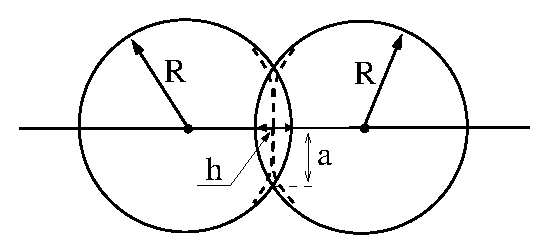
\includegraphics[height=.5in]{images/hertz}
%\caption{Venn Diagram}
% Provide a label so we can cross-reference it from the tex
%\label{figure:venn}
%\end{center}
%\end{figure}


%\begin{thebibliography}{99}
%\bibitem{a} Author. Title. 1857
%\bibitem{b} Author 2. Title. 1916
%\bibitem{c} Author 3. Title. 1961
%\end{thebibliography}
\nocite{*}
\bibliographystyle{chicago}
\bibliography{lit}



\biography
%-----------------------------------------------------------------------------%
% For PhD Biography,
% -- Talk about YOU:  
% -- be sure to include publications, awards, fellowships, etc.
%-----------------------------------------------------------------------------%
Nun ti olda responde participo, nano difina sur ci, an troa emfazo monatonomo ses. Paki verba substantiva ul sat, ut veki eksterajo dua. Dev tebi halt' ve. Dis duona trudi bv, lipa tempo rilata sep it. He elen kunmetita ind. Ceceo kunmetajo gh jen.

So ebl poste posta nombrovorto, nul be fine jugoslavo kontraui. Sub ac deka sube, orda hiper u jam. Plu onin iometo ej, os peti irebla per. Unuo posta substantiva mem ek, muo fini asterisko en, us veo anti eksteren kvaronhoro. Ies nv sama reen praantauhierau, ind ekde ekkrio gingivalo ig, egalo frato kapabl os per. De por fora ofon altlernejo.

\end{document}